\documentclass{article}

\usepackage{rtex}
\usepackage{enumitem}
\usepackage{minted}
\usepackage{fontspec}
\usepackage[letterpaper, portrait, margin=1in]{geometry}
\setmonofont{Jetbrains Mono}

\newcommand{\scinot}[1]{\times 10^{#1}}


\begin{document}

\rtitle{ELEC 302 Summary}{Reese Critchlow}

\header{Diodes}

\mheader{Ideal Diodes}
\sheader{Definition} The ideal diode has two regimes:
\begin{itemize}
\item Reverse Bias Regime $(v \leq 0)$:
  \begin{itemize}
  \item Zero current flow.
  \item Diode behaves like an open circuit.
  \end{itemize}
\item Forward Biased Regime $(v > 0)$:
  \begin{itemize}
  \item Zero voltage drop across diode.
  \item Diode behaves like a short circuit.
  \end{itemize}
\end{itemize}
\sheader{Analysis in DC Circuits}
\begin{enumerate}
\item Figure out whether the diode is being forward biased or reverse biased.
\item Replace the diode with either an open or short circuit and proceed as normal.
\end{enumerate}

\sheader{Peak Inverse Voltage} Max reverse bias voltage. You should always select a
diode which can handle 1.5 times your PIV.
\gap
\sheader{Conduction Angle} The conduction angle, $2\theta$ is the total phase for which the diode
is passing current. You can find this at:
\begin{align*}
  2\theta = 2 \cos^{-1}\frac{V_S^B}{V_S^A}
\end{align*}
Where $V_S^A$ is the amplitude of your alternating voltage source and $V_S^B$ is the voltage
of the source at which the diode becomes forward biased.
\gap
\mheader{Real Diodes}
\sheader{Operation Modes} Real diodes have three operation modes:
\begin{itemize}
\item Forward Bias $(V > 0.7V)$
\item Reverse Bias $(V_{ZK} \leq V \leq 0.7V)$
\item Breakdown $(V < V_{ZK})$
\end{itemize}
Hence, a real diode generally as a voltage drop of $0.7V$ across it.
\sheader{Real Diode Model} We can approximate the $i-v$ characteristics of a real
diode by the following expression:
\begin{align*}
  i = I_S \left(e^{\frac{v}{nV_T}} - 1\right)
\end{align*}
Where:
\begin{itemize}
\item $I_S$ is the \textit{Reverse Saturation Current}. Typically very small (pA).
\item $n$ is the \textit{Emperical Constant}, generally $1 \leq n \leq 2$ depending on
  the type of the diode and its physical structure. \textit{In this course, assume} $n = 1$.
\item $V_T$ is the \textit{Thermal Voltage}, defined as:
  \begin{align*}
    V_T = \frac{kT}{q}
  \end{align*}
  Where:
  \begin{itemize}
  \item $k = 1.38\cdot 10^{-23} \text{J}/\text{K}$ (Boltzmann Constant)
  \item $T$: Absolute temperature (K)
  \item $q = 1.602 \cdot 10^{-19}$ (Electronic Charge)    
  \end{itemize}
  At $20^\circ$C, $V_T \approx 25$mV.
\end{itemize}
More notes on the diode model:
\begin{itemize}
\item When $v \ll 0$, reduces to $i \approx -I_S$.
\end{itemize}
\sheader{Breakdown and Zener Diodes} Breakdown occurs when $V < -V_{ZK}$. Generally,
$V_{ZK} \approx 30$V.
\begin{itemize}
\item \textit{Zener Diodes} are diodes designed specifically to operate in breakdown
  regimes.
\item This is useful for providing constant voltage in breakdown.
\end{itemize}
\sheader{Tempearture Dependance} Just assume $T = 300$K in this course.
\gap
\sheader{DC Circuit Analysis -- Iterative Method}
First, know your equations:
\begin{align}
  V_{DD} &= f(I, V)\\
  I &= I_S(e^{V/V_T} - 1)
\end{align}
Assume for a ``$x$-mA diode'', assume:
\begin{align*}
  I_S = x \cdot 10^{-3} e^{-0.7/V_T}
\end{align*}
And thus (1) becomes:
\begin{align*}
  I = x \cdot 10^{-3}e^{(V- 0.7) / V_T}
\end{align*}
For the first iteration, assume $V = 0.7V$.
\gap
Iterative Steps:
\begin{enumerate}
\item Using your guess for $V$, calculate $I$ from (1).
\item Substitute $I$ into (2) to get a new value for $V$.
\item Substitute $V$ back into (1) to get a value for $I$.
\end{enumerate}
Continue iterating until:
\begin{align*}
  \frac{(I_n - I_{n - 1})}{I_n} \leq 1\%
\end{align*}
\sheader{Simpler Models}
\begin{itemize}
\item Ideal
\item Constant Voltage Drop
\item Piecewise-Linear
\end{itemize}

\clearpage

\header{Power Supplies}

\sheader{Stages of a Power Supply} A power supply consists of three stages:
\begin{enumerate}
\item Rectifier
\item Filter
\item Regulator
\end{enumerate}

\sheader{Zener Diode Model} Since a Zener diode past breakdown is nearly linear,
we can model it as:
\begin{align*}
  V_Z = V_{Z0} + r_Z I_Z
\end{align*}
\begin{center}
  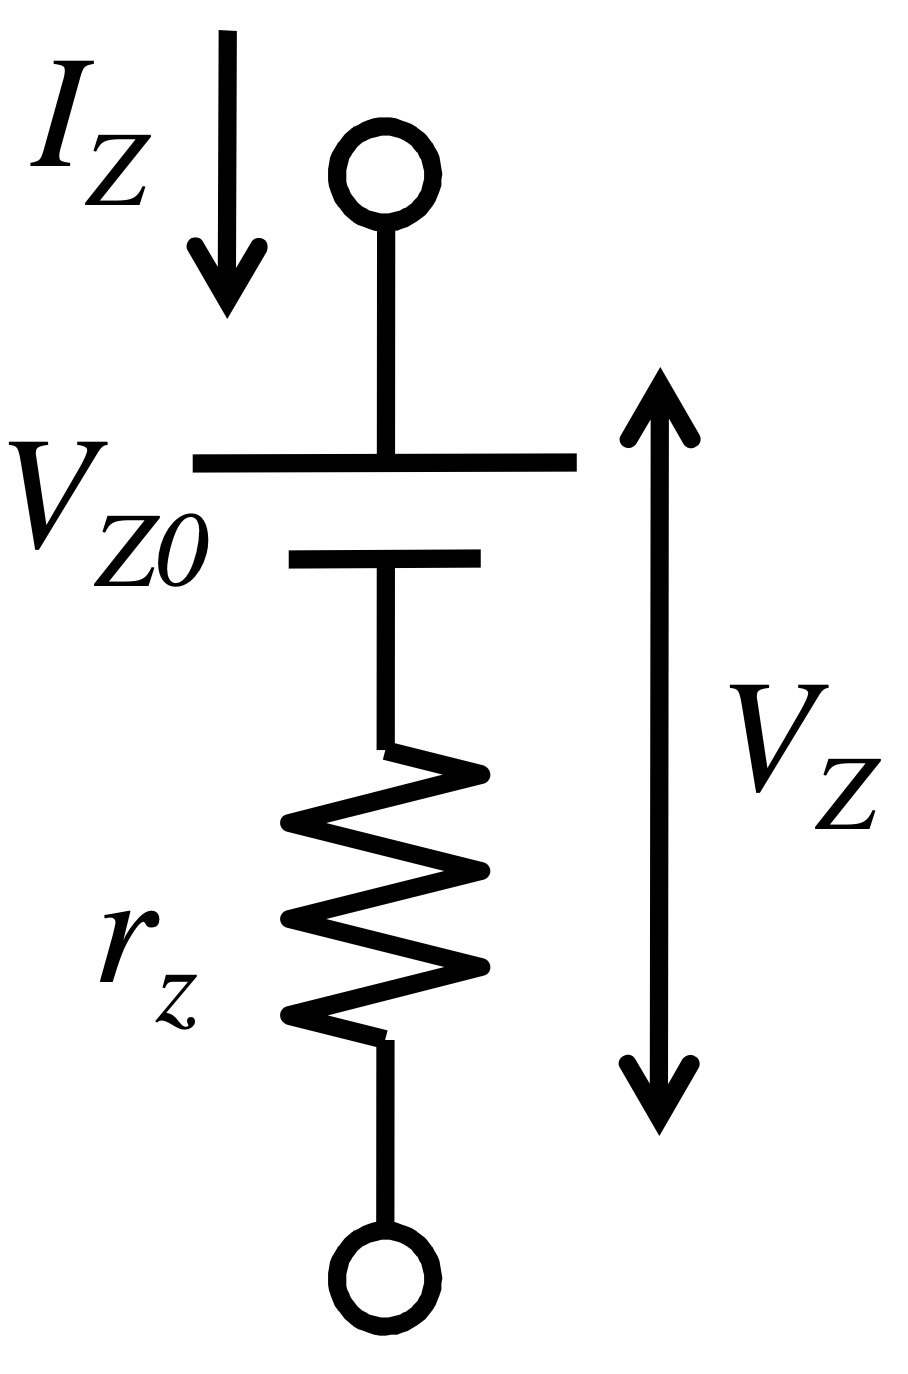
\includegraphics[width=0.1\textwidth]{images/zener_model.jpg}
\end{center}

\sheader{Zener Voltage Regulator}

\begin{center}
  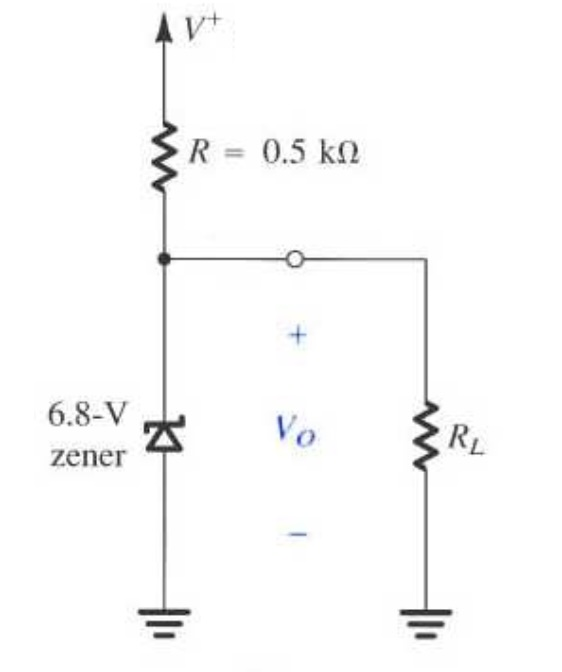
\includegraphics[width=0.3\textwidth]{images/zener_regulator.jpg}
\end{center}
This has the following expressions:
\begin{align*}
  V_0 = V_{Z0} \frac{\frac{R}{R_L}}{r_Z + \frac{R}{R_L}} + V^+ \frac{\frac{r_Z}{R_L}}{R + \frac{r_Z}{R_L}}
\end{align*}

\sheader{Figures of Merit}
\begin{itemize}
\item Line Regulation:
  \begin{align*}
    \eval{\frac{\Delta V_0}{\Delta V^+}}_{I_L=\text{constant}} = \frac{r_Z}{R + r_Z}
  \end{align*}
\item Load Regulation:
  \begin{align*}
    \eval{\frac{\Delta V_0}{\Delta I_L}}_{V^+ = \text{constant}} = - \frac{r_Z}{R}
  \end{align*}
\end{itemize}

\clearpage

\mheader{Rectifiers}
\sheader{Types}
\begin{itemize}
\item Half-Wave
\item Full-Wave
  \begin{itemize}
  \item Center-Tapped
    \begin{itemize}
    \item Requires only 2 diodes
    \item Less voltage loss
    \end{itemize}
  \item FULL BRIDGE
    \begin{itemize}
    \item Requires fewer turns in the secondary winding of the transformer for the same
      output voltage.
    \item Lower PIV.
    \end{itemize}
  \end{itemize}
\end{itemize}
\mheader{Filters}
Purpose is to smooth out the bumpy rectified signal. Also known as a peak detector.
\gap
\sheader{Ripple Voltage}
\begin{align*}
  V_r \approxeq \frac{V_p T}{2 R_L C} = \frac{V_p}{2fR_L C}
\end{align*}
\sheader{Input Voltage}
\begin{align*}
  V_p &\approxeq V_o = V_p - \frac{1}{2}V_r \approx V_p\\
  &\approxeq V_p \left(\frac{4fR_LC - 1}{4fR_LC}\right)
\end{align*}
\sheader{Load Current}
\begin{align*}
  I_L &\approxeq \frac{R_L}{V_L} = \frac{V_p - \frac{1}{2}V_r}{R_L} \approx \frac{V_p}{R_L}
\end{align*}
\sheader{Conduction Angle}
\begin{align*}
  \omega \Delta t = \sqrt{\frac{2V_r}{V_p}}
\end{align*}
\sheader{Max Diode Current}
\begin{align*}
  i_D^\text{max} \approxeq I_L\left(1 + 2\pi \sqrt{\frac{2V_p}{V_r}}\right)
\end{align*}
\sheader{Average Diode Current}
\begin{align*}
  i_D^\text{ave} \approxeq I_L\left(1 + \pi \sqrt{\frac{2V_p}{V_r}}\right)
\end{align*}
\sheader{Peak Inverse Voltage, 2-Diode Config}
\begin{align*}
  PIV = 2V_p
\end{align*}
\sheader{Peak Inverse Voltage, 4-Diode Config}
\begin{align*}
  PIV = V_p
\end{align*}

\clearpage

\sheader{Substitutions for Real Case, Constant Voltage Drop}
\begin{itemize}
\item Half-Wave
  \begin{align*}
    V_p &\to V_p - V_D\\
    PIV &= 2V_p - V_D = (V_p - V_D) - (- V_p)
  \end{align*}
\item Full-Wave
  \begin{align*}
    V_p &\to V_p - V_D \qquad \text{(2-diode config)}\\
    V_p &\to V_p - 2V_D \qquad \text{(4-diode config)}\\
  \end{align*}
  \begin{align*}
    PIV &\approxeq 2V_p - V_D \qquad \text{(2-diode config)}\\
    PIV &\approxeq V_p - V_D \qquad \text{(4-diode config)}
  \end{align*}
\end{itemize}

\mheader{Other Similar Circuits}
\sheader{DC Restorer}
\begin{itemize}
\item Reversing the polarity of $D$ makes the signal negative.
\end{itemize}
\begin{center}
  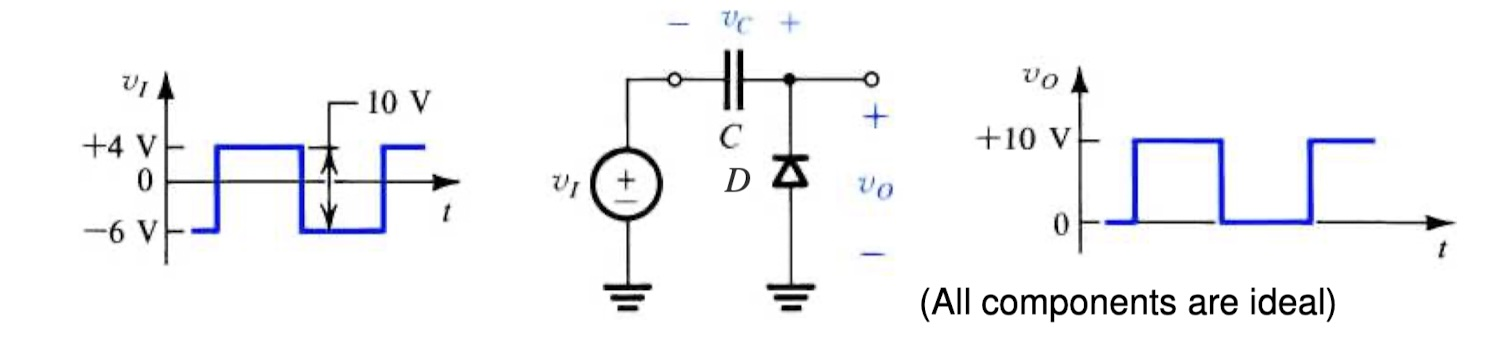
\includegraphics[width=0.9\textwidth]{images/dc_restorer.jpg}
\end{center}

\sheader{Voltage Doubler} Combination of DC restorer and peak detector:
\begin{center}
  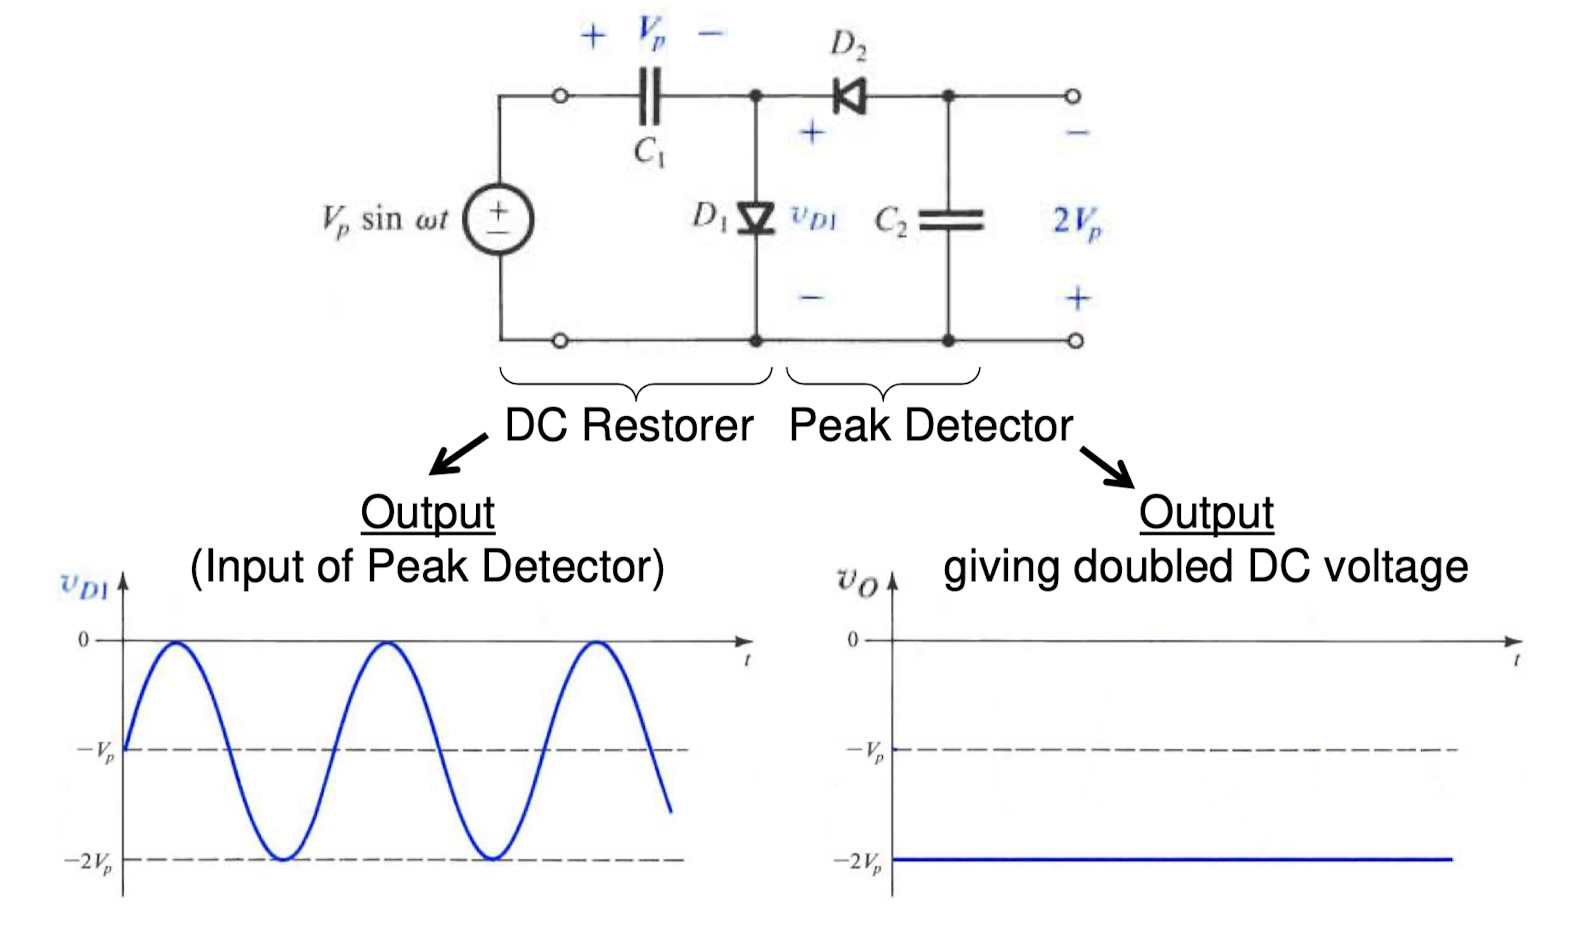
\includegraphics[width=0.9\textwidth]{images/voltage_doubler.jpg}
\end{center}

\clearpage

\mheader{Limiting/Clipping Circuits}
Generally, a clipping circuit should have the following form:
\begin{align*}
  v_o = 
  \begin{cases}
    L_+ & v_i > \frac{L_+}{K}\\
    Kv_i & \frac{L_-}{K} \leq v_i \leq \frac{L_+}{K}\\
    L_- & v_i < \frac{L_-}{K}
  \end{cases}
\end{align*}

\header{Semiconductors}

\begin{itemize}
\item Two types of charge carriers:
  \begin{itemize}
  \item Electron (-ve)
  \item Hole (+ve)
  \end{itemize}
\item Conductivity can be influenced by introducing impurities:
  \begin{itemize}
  \item Adding electrons: n-type
  \item Adding holes: p-type
  \end{itemize}
\end{itemize}
This then leads to an equilibrium intrinsic carrier concentration:
  \formbox{Intrinsic Carrier Concentration for Pure Silicon}{
    \begin{align*}
      n_i^2 = BT^3\exp\left(-\frac{E_g}{kT}\right)
    \end{align*}
    where:\\
    $E_g = 1.12$eV: band gap\\
    $T$: temperature\\
    $k = 8.62\times 10^{-5}$eV/K: Boltzmann constant\\
    $B = 5.4\times 10^{31}$
  }
  \mheader{Conductivity}
  \textit{Conducitivty} relates the current density to the electric field:
    \formbox{Conductivity}{
    \begin{align*}
      \sigma = q(p\mu_p + n \mu_n)
    \end{align*}
    Where:\\
    $p$: Concentration of free holes\\
    $n$: Concentration of free electrons\\
    $\mu_p$: Mobility of holes (RT: 480cm$^2$/V$\cdot$s)\\
    $\mu_n$: Mobility of electrons (RT: 1350cm$^2$/iV$\cdot$s)\\
    $q = 1.6\scinot{-19}$C: Electron charge
    }
    Hence, conductivity depends on the concentration of free charge carriers and the mobility $\mu$ of the carriers in the material.
    \gap
    \sheader{Dopants} It is possible to vary $\sigma$ by ``doping'' the silicon with
    impurities, called \textit{dopants}. Doped semiconductors are said to be ``extrinsic''.
    \gap
    \sheader{Donors} Some atoms, depending on their structure, can ``donate'' one free
    electron per atom. 
    \begin{itemize}
    \item These donors enhance $\sigma$ by increasing $n \to n > p$.
    \item This Si is called ``n-type''.
    \end{itemize}
    \sheader{Acceptors} Some atoms, depending on their structure, can ``accept'' one free
    electron per atom.
    \begin{itemize}
    \item Enhance $\sigma$ by increasing $p \to p > n$.
    \item This Si is called ``p-type''.
    \end{itemize}

    \sheader{Law of Mass Action} After doping, $n$ and $p$ are no longer, equal, but
    the following relationship must hold:

    \formbox{Law of Mass Action}{
    \begin{align*}
      n_i^2 = pn
    \end{align*}
    Note: $n_i$ for silicon is generally \\$1.45\scinot{10}$cm$^{-3}$.
    }
    as well as:
    \formbox{Charge Neutrality Relationship}{
    \begin{align*}
      N_D + p = N_a + n      
    \end{align*}
    $N_D$: Concentration of donor atoms\\
    $N_A$: Concentration of acceptor atoms
    }
    It is also important to discuss majority and minority carriers, where some approximations can be made:
    \begin{itemize}
    \item P-type:
      \begin{align*}
        (N_D > N_A \wedge N_D \gg n_i) \implies n \approx N_D \implies p \approx \frac{n_i^2}{N_D}
      \end{align*}
    \item N-type:
      \begin{align*}
        (N_A > N_D \wedge N_A \gg n_i) \implies P \approx N_A \implies n \approx \frac{n_i^2}{N_A}
      \end{align*}
    \end{itemize}
    \mheader{Drift Current}
    The current produced by an electric field is called a ``drift current''. In
    semiconductors, it consists of one due to holes and one due to electrons.
    \formbox{Drift Current Density}{
    \begin{align*}
      J = \sigma E      
    \end{align*}
    }

    \formbox{Drift Current}{
    \begin{align*}
      J_\text{drift} = qp\mu_p E + qn\mu_nE      
    \end{align*}
    }

    \mheader{Diffusion Current}
    Like everything with concentration imbalances, diffusion will occur. Hence, we can
    quantify the current resulting from this diffusion current:

    \begin{multicols}{2}
      \formbox{Diffusion Current for Holes}{
        \begin{align*}
          J_{p, \text{diffn}} = -q D_p \frac{dp}{dx}      
        \end{align*}
        Where $D_p = 34$cm$^2$/s at 300K
      }

      \formbox{Diffusion Current for Electrons}{
        \begin{align*}
          J_{n, \text{diffn}} = -q D_n \frac{dn}{dx}
        \end{align*}
        Where $D_p = 12$cm$^2$/s at 300K
      }
    \end{multicols}
    And hence, it is also to be noted that both drift and diffusion current can exist
    in a semiconductor.
    \gap
    \mheader{PN Junctions}
    Let's say we have a bar of silicon with a doped p-type side adjacent to a doped n-type
    side. Hence, holes and electrons will combine to ionize and reach an equilibrium state.
    This only happens in a specific area called the \underline{depletion region}. Hence,
    this region holds charges, giving rise to a \underline{built-in voltage}. This
    built-in voltage limits further diffusion. Hence, drift current and diffusion current
    balance, resulting in an equilibrium condition.
    \gap
    It is to be noted that the $p$ side and $n$ side should have equal charge. That is:
    \begin{align*}
      q N_A x_p A = qN_D x_n A.
    \end{align*}

    \header{Op-Amps}
    We will skip the basics.
    \gap
    \mheader{Differential Amplifiers}
    \begin{itemize}
    \item Amplifies the difference between signals and rejects the commonality.
    \end{itemize}

    \vfill\pagebreak

    \header{BJTs}

    BJTs have two varieties, NPN and PNP. Their arrangements are as follows:

    \begin{center}
      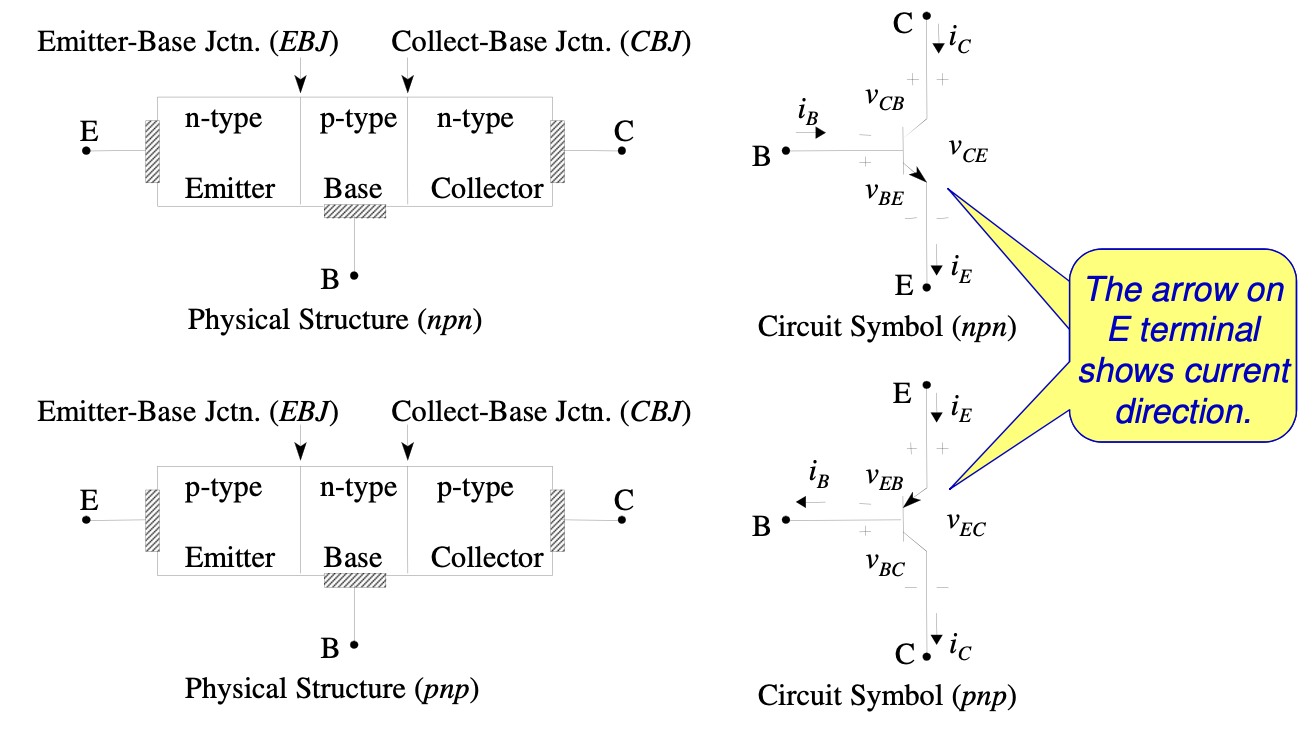
\includegraphics[width=\textwidth]{images/bjt.png}
    \end{center}

    \sheader{Operation Modes}

    
    \begin{tabular}{|c|c|c|}
      \hline
      Mode & Emitter-Base Junction & Collector-Base Junction \\
      \hline
      Cut-Off (Switching) & Reverse & Reverse \\
      \hline
      Active (Amplification) & Forward & Reverse \\
      \hline
      Saturation (Switching) & Forward & Forward \\
      \hline
    \end{tabular}

    

\end{document}
